%
% ME4140 - Fall 2016 - Fall 2020
% ROS by Tristan Hill - Tutorials for TnTech Students
% Tutorial 1 - Virtualizing Ubuntu
%

\documentclass[12pt]{article}
\usepackage{hyperref}
\usepackage[pdftex]{graphicx}
\usepackage{multirow}
\usepackage{setspace}
\usepackage{color}
\usepackage{multicol}
\usepackage{enumitem}

\hypersetup{
    bookmarks=true,         % show bookmarks bar?
    unicode=false,          % non-Latin characters in Acrobat’s bookmarks
    pdftoolbar=true,        % show Acrobat’s toolbar?
    pdfmenubar=true,        % show Acrobat’s menu?
    pdffitwindow=false,     % window fit to page when opened
    pdfstartview={FitH},    % fits the width of the page to the window
    pdftitle={My title},    % title
    pdfauthor={Author},     % author
    pdfsubject={Subject},   % subject of the document
    pdfcreator={Creator},   % creator of the document
    pdfproducer={Producer}, % producer of the document
    pdfkeywords={keyword1, key2, key3}, % list of keywords
    pdfnewwindow=true,      % links in new PDF window
    colorlinks=true,       % false: boxed links; true: colored links
    linkcolor=red,          % color of internal links (change box color with linkbordercolor)
    citecolor=green,        % color of links to bibliography
    filecolor=magenta,      % color of file links
    urlcolor=blue           % color of external links
}

% custom colors
\definecolor{TTUpurple}{rgb}{0.3098, 0.1607, 0.5176} % TTU Purple (primary)
\definecolor{TTUgold}{rgb}{1.0000, 0.8666, 0.0000} % TTU Gold (primary) 
\definecolor{mygray}{rgb}{.6, .6, .6}
\definecolor{mypurple}{rgb}{0.6,0.1961,0.8}
\definecolor{mybrown}{rgb}{0.5451,0.2706,0.0745}
\definecolor{mygreen}{rgb}{0, .39, 0}
\definecolor{mypink}{rgb}{0.9960, 0, 0.9960}

% color commands
\newcommand{\R}{\color{red}}
\newcommand{\B}{\color{blue}}
\newcommand{\BR}{\color{mybrown}}
\newcommand{\K}{\color{black}}
\newcommand{\G}{\color{mygreen}}
\newcommand{\PR}{\color{mypurple}}
\newcommand{\PN}{\color{mypink}}
\newcommand{\OR}{\color{TTU}}
\newcommand{\GD}{\color{TTUgold}}

\newcommand{\Lagr}{\mathcal{L}} % lagrangian

\newcommand{\hspcu}{\underline{\hspace{20mm}}} % large horizontal space w underline
\newcommand{\vspccc}{\vspace{6mm}\\} % large vertical space
\newcommand{\vspcc}{\vspace{4mm}\\}   % medium vertical space
\newcommand{\vspc}{\vspace{2mm}\\}     % small vertical space

\newcommand{\hspcccc}{\hspace{10mm}} % large horizontal space
\newcommand{\hspccc}{\hspace{6mm}} % large horizontal space
\newcommand{\hspcc}{\hspace{4mm}}   % medium horizontal space
\newcommand{\hspc}{\hspace{2mm}}     % small horizontal space

\newsavebox{\mybox} % custom box

\textwidth=6.5in
\topmargin=-0.5in
\textheight=9.25in
\hoffset=-0.5in
\footskip=0.2in

\pagestyle{myheadings}
\markright{{\large ME 4140 Fall 2020 - Tutorial 1 - Virtualize Ubuntu}}

\newcommand{\homeWeight}{10}
\newcommand{\quizWeight}{20}
\newcommand{\examWeight}{15}
\newcommand{\finalWeight}{25}

\begin{document}

\thispagestyle{plain}

\begin{center}
   {\bf \Large ROS Workshop - Tutorial 1 - Virtualize Ubuntu}\vspace{3mm} \\
   {\bf \large ME 4140 - Introduction to Robotics - Fall 2020} \vspace{5mm}\\
\end{center}

\begin{description}

 	\item[\underline{What is a \href{https://en.wikipedia.org/wiki/Virtual_machine}{Virtual Machine} ?}]: \\
 	\begin{multicols}{2}
      		
            \begin{itemize}
                
                \item A virtual machine is an operating system that is installed or {\it virtualized} inside another operating system.
                \item This is useful for learning and testing, but it is resource intensive and is not ideal for permanent use. 
                \item \href{https://www.virtualbox.org/}{VirtualBox} is a trusted application commonly used for this process
                
            \end{itemize}
            
\includegraphics[scale=.15]{CaptureA.png}\\
	\end{multicols}
	
	\item[\underline{Overview}]: \vspace{0mm} \\

		        You will first download and install VirtualBox from Oracle which is an application for {\it virtualizing} operating systems on top of an existing one. Next you will download the Ubuntu installation .iso file and setup a virtual operating system for learning ROS.  After completing this exercise, you will be ready to install the ROS Melodic software package in Ubuntu which is described in detailed in the next module. 

	\item[\underline{System Requirements}]: \vspace{0mm} \\

		        \begin{itemize}

					\item {\bf CPU:} Most modern notebook or desktop computers will work well. If you are using a very old computer it may be very slow. A tablet or Chromebook is not supported.
					\item {\bf Memory:} At least 8Gb of RAM is recommended.        
                    \item {\bf Storage:} Approximately 20Gb of free space on a hard drive is required. This space will remain in its current partition, and you are free to delete the files later. USB 2.0 or slower connection to the hard drive is not recommended. 
    
                \end{itemize}
                
			\item[\underline{Disclaimer}]: 
			\begin{itemize}
			
				\item {\bf \R It is a good idea to back up any important files before you begin a project. Hard disk drives fail. Solid state drives can also fail. } 
				\item Some students may have to adjust a computer BIOS setting to allow virtualization. This setting can be easily reverted.   
				\item It is recommended to have your computer's power supply available before you begin this installation process. 
			
			\end{itemize} 			
			
			
                    
  

\newpage

\item[\underline{Detailed Setup Process}]: 

\begin{description} 
	

\item [Part 1 - Install VirtualBox Application]: \vspace{0mm}\\ 


\begin{enumerate}[label=\alph*)]
	
	\item Download the VirtualBox installation file using the link on ilearn. Choose the link that matches your computer type. If you are using a Linux computer already you do not need this tutorial. \vspace{5mm}
	
	\item Click the VirtualBox installation file you downloaded and install the application. You will need to provide admistrator access and click allow. You no longer need the installation file, but it is small so it wont hurt to keep it. \vspace{5mm} \\
	
	\hspace*{-2.5cm}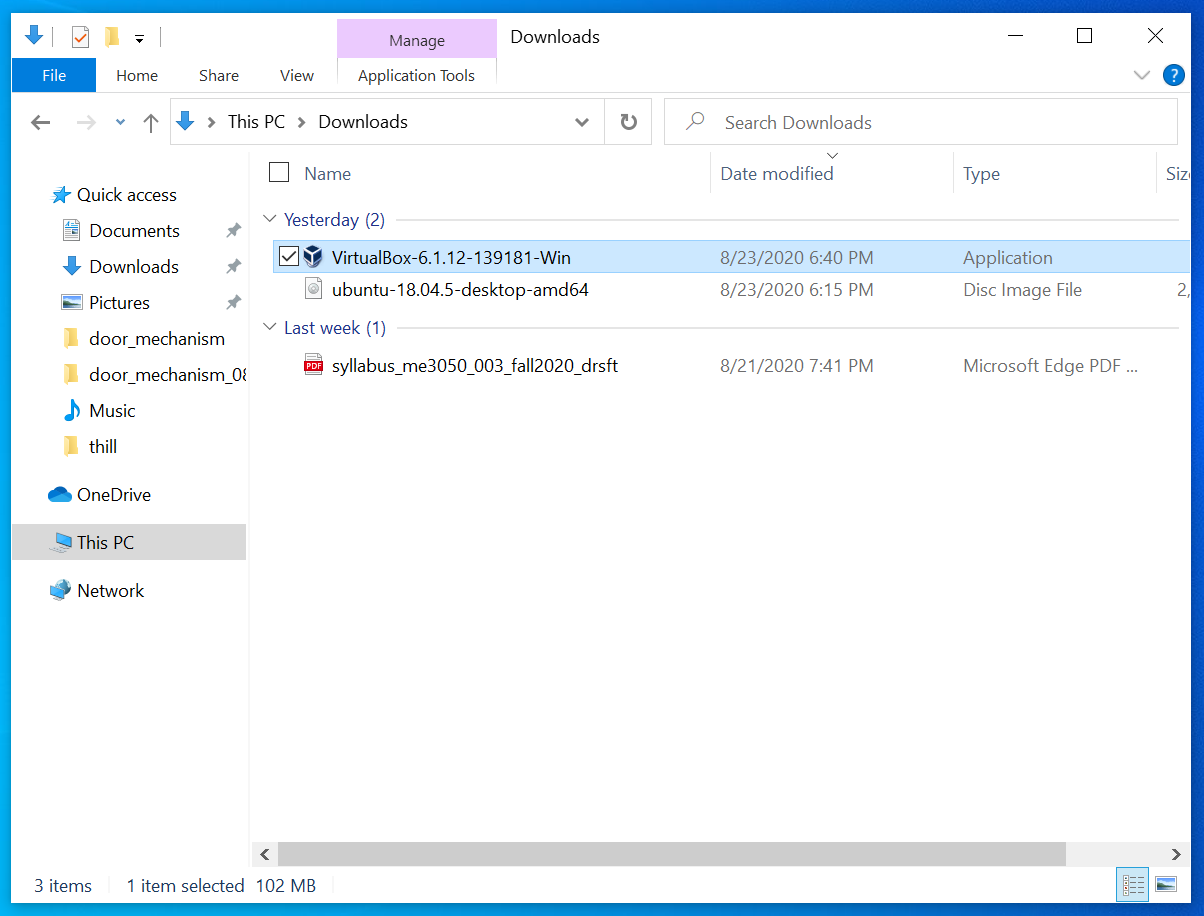
\includegraphics[scale=.6]{Capture1.png}\\

\end{enumerate}
  
  
\newpage  
\item [Part 2 - Virtual Machine Configuration]: \vspace{0mm} \\
\begin{enumerate}[label=\alph*)] 
    	\item Open the VirtualBox application you installed in step 2. \vspace{5mm} \\
    	\begin{multicols}{2}
      	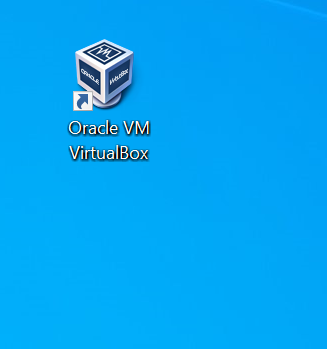
\includegraphics[scale=.55]{Capture2.png}\\
          
                
                before proceeding make sure you have an {\bf \B internet connection } access to a {\bf \R power supply or battery }
         
            \end{multicols}
            \vspace{10mm}
       

	\item Create New Virtual Machine:  \vspace{5mm} \\
      		\hspace*{-2.5cm}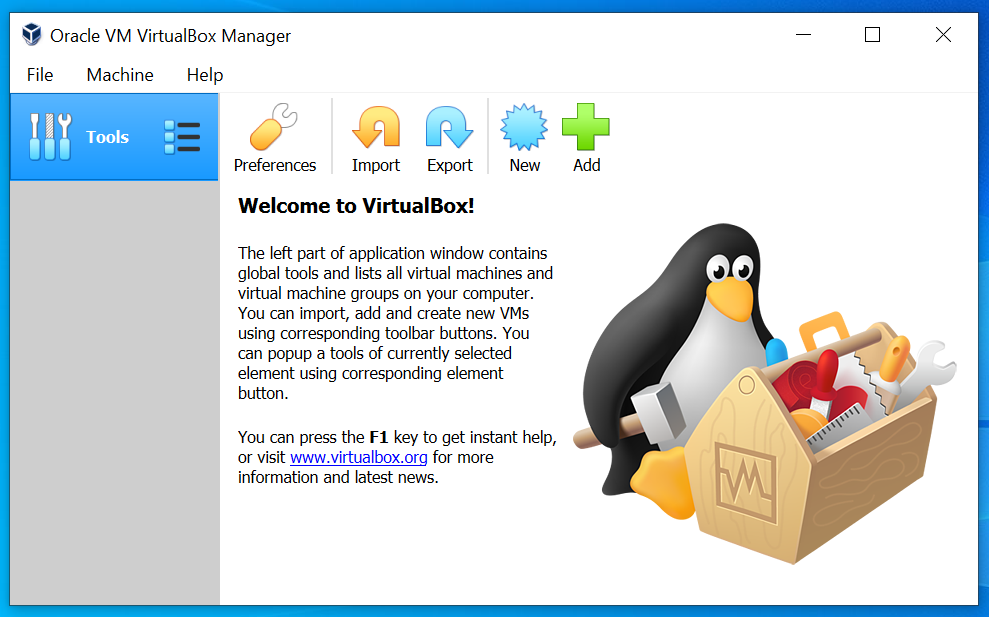
\includegraphics[scale=.55]{Capture3.png}\\
               \begin{itemize}
                
	\item press the {\bf new} button

                
            \end{itemize}
   
   \newpage         
          \item Define Basic Settings:  \vspace{5mm} \\  
            \hspace*{-2.5cm}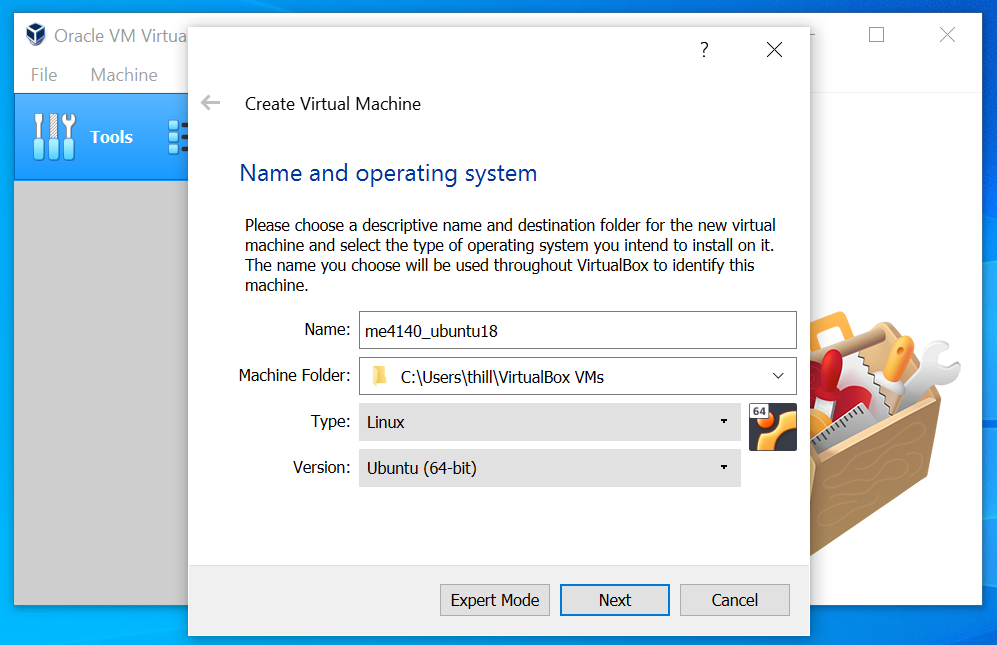
\includegraphics[scale=.55]{Capture4.png}\\
\begin{itemize}
                
                \item choose a {\bf computer name} (this is your choice but remember it!)
                \item choose an {\bf operating system} type (Linux)
                \item choose a {\bf version}, this depends on your physical machine - probably Ubuntu 64-bit 
                \item click {\bf next}
                
            \end{itemize}
\vspace{10mm}
\item Define Virtual Machine Parameters: \vspace{5mm} \\
      		\hspace*{-2.5cm}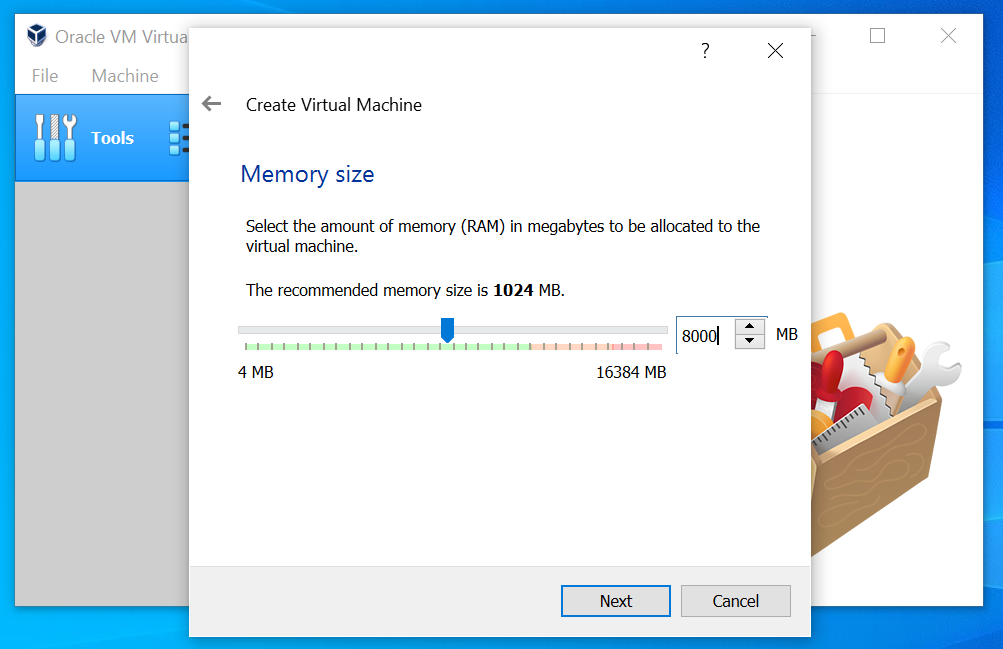
\includegraphics[scale=.55]{Capture5.png}\\
            \begin{itemize}
                
                \item Choose the amount of RAM you want to allocate to the VM  
                \item More is better but you must leave some RAM for the host operating system (Windows or Mac). If your computer has 8GB total I suggest no more than 6GB for for the virtual machine.  
                \item click {\bf next}
                
            \end{itemize}

\newpage
\item Define Virtual Hard Drive Parameters: \vspace{5mm} \\
      		\hspace*{-2.5cm}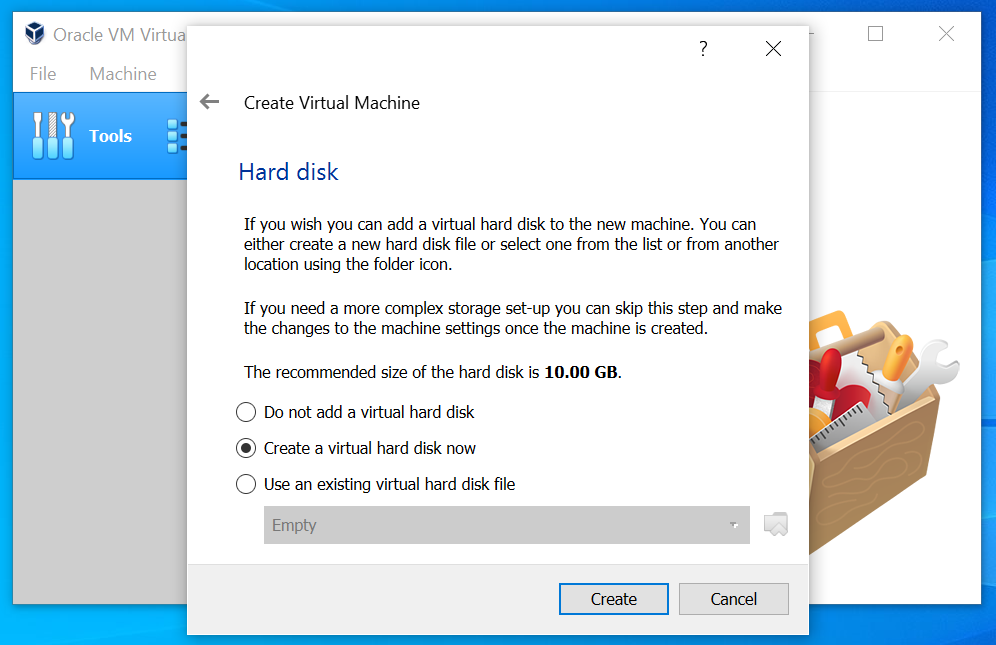
\includegraphics[scale=.55]{Capture6.png}\\
 \begin{itemize}
                
       
                \item choose {\bf create a virtual hard drive now}
                \item click {\bf create}
                
                
            \end{itemize}
\vspace{10mm}
\item Virtual Hard Drive Setup: \vspace{5mm} \\

        \hspace*{-2.5cm}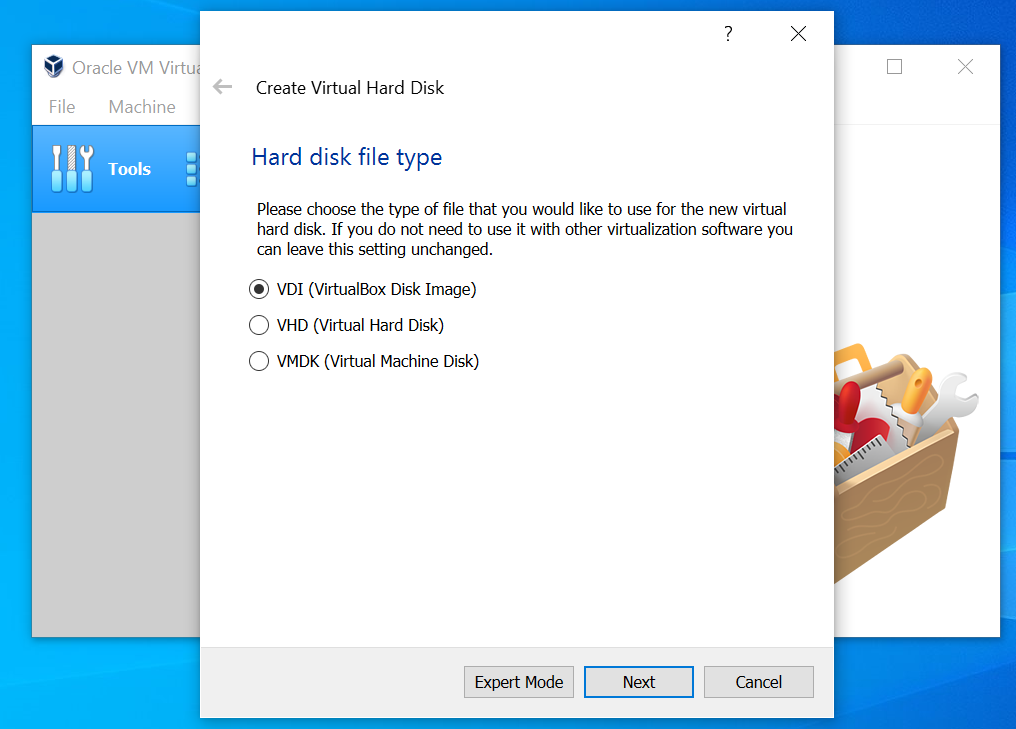
\includegraphics[scale=.55]{Capture7.png}\\
        \begin{itemize}
                        
                \item choose the virtual hard drive type, VDI is recommended. 
                \item click {\bf next}
                           
        \end{itemize}

\newpage
\item Virtual Hard Drive Setup: \vspace{5mm} \\

      		\hspace*{-2.5cm}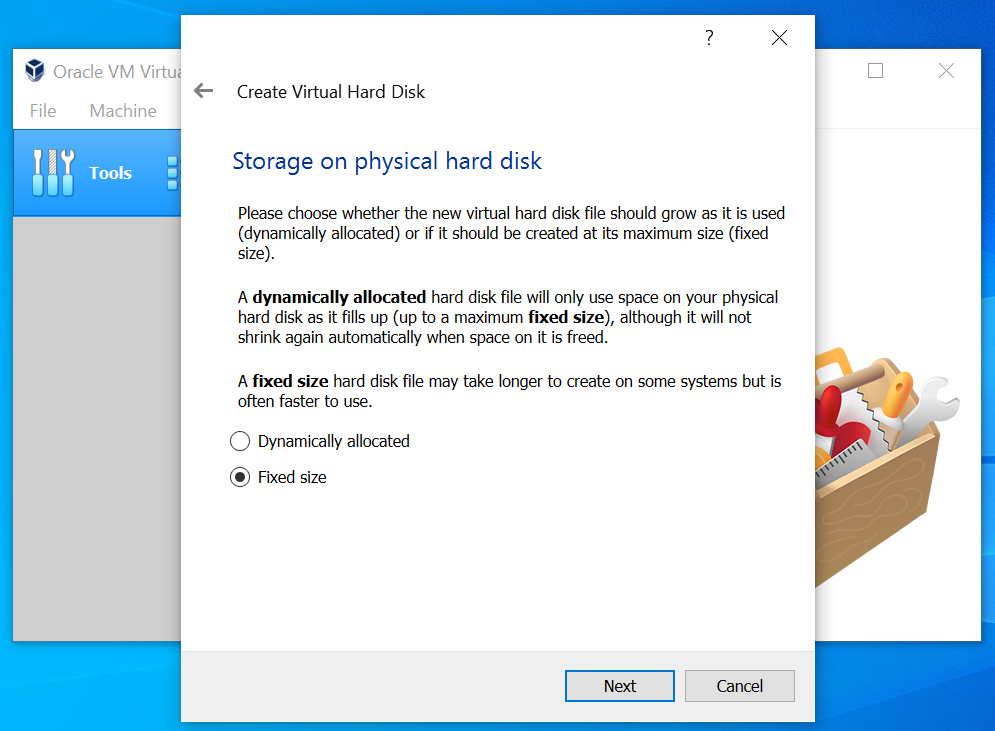
\includegraphics[scale=.55]{Capture8.png}\\
            \begin{itemize}
                
                \item choose {\bf Fixed size} virtual hard drive. 
                \item click {\bf next}
                              
            \end{itemize}

\vspace{10mm}
\item Virtual Hard Drive Setup : \vspace{5mm} \\
      		\hspace*{-2.5cm}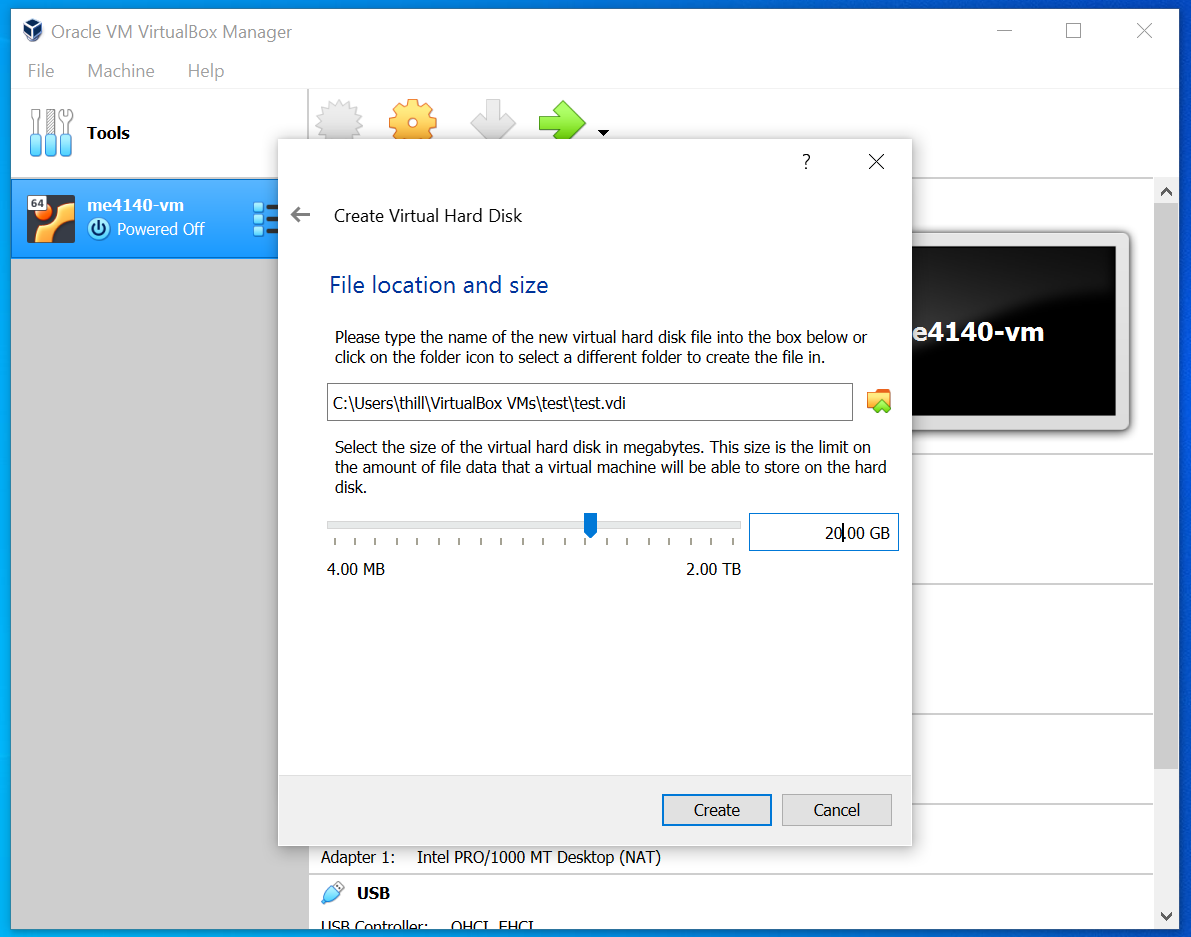
\includegraphics[scale=.50]{CaptureX.png}\\
             \begin{itemize}
                    
                \item choose the size of your virtual hard drive       
                \item to virtualize Ubuntu and install ROS it is recommended to make a 20 GB VDI if you have space
                \item click {\bf create}
          
            
                
            \end{itemize}
	\newpage

     \end{enumerate}

\item[Part 3 - Ubuntu OS Installation and Setup]: \vspace{5mm} \\

\begin{enumerate}[label=\alph*)] 
\item Start the VM for the first time: \vspace{5mm} \\
      		\hspace*{-2.5cm}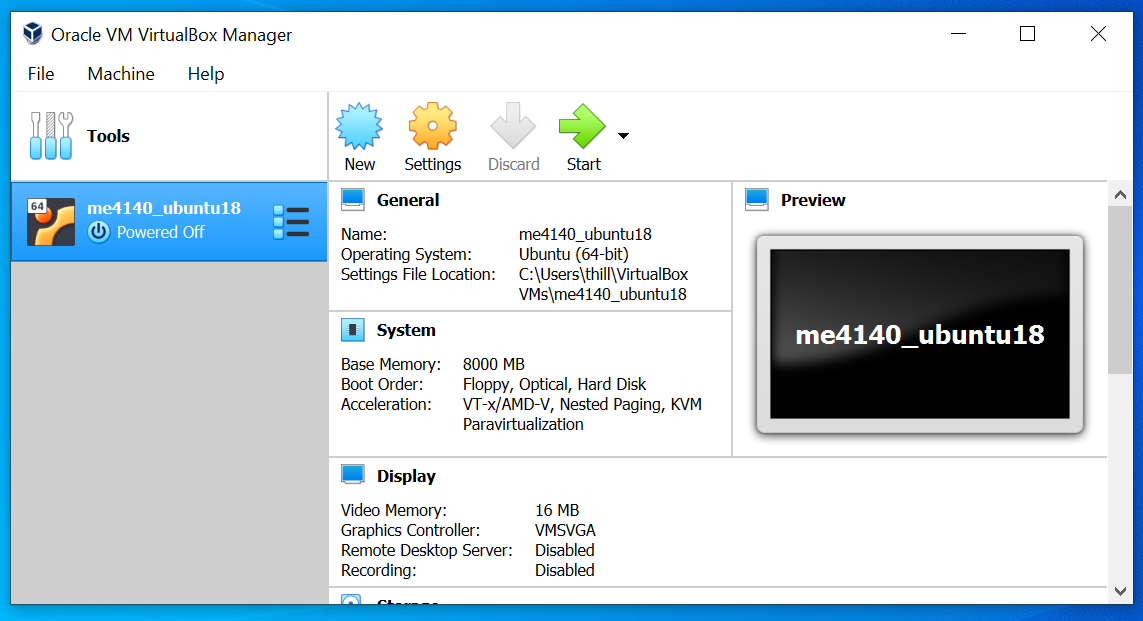
\includegraphics[scale=.6]{Capture9.png}\\
            \begin{itemize}
                    
                 \item select your newly created VM      
                 \item press the green {\bf start} button and wait...
     
            \end{itemize}
\vspace{10mm}
\item Find the folder icon: \vspace{5mm} \\
      		\hspace*{-2.5cm}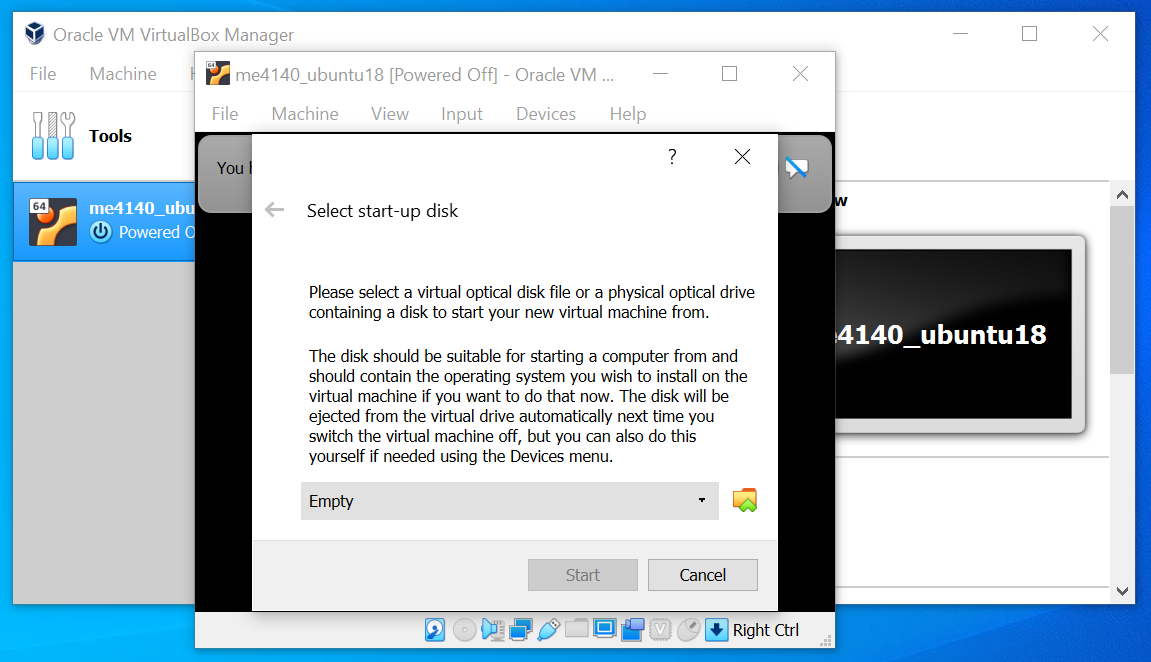
\includegraphics[scale=.6]{Capture10.png}\\
            \begin{itemize}
                    
                 \item choose to select media from a local folder 
                 
            \end{itemize}

\newpage	
\item Choose the installation media: \vspace{5mm} \\
      		\hspace*{-2.5cm}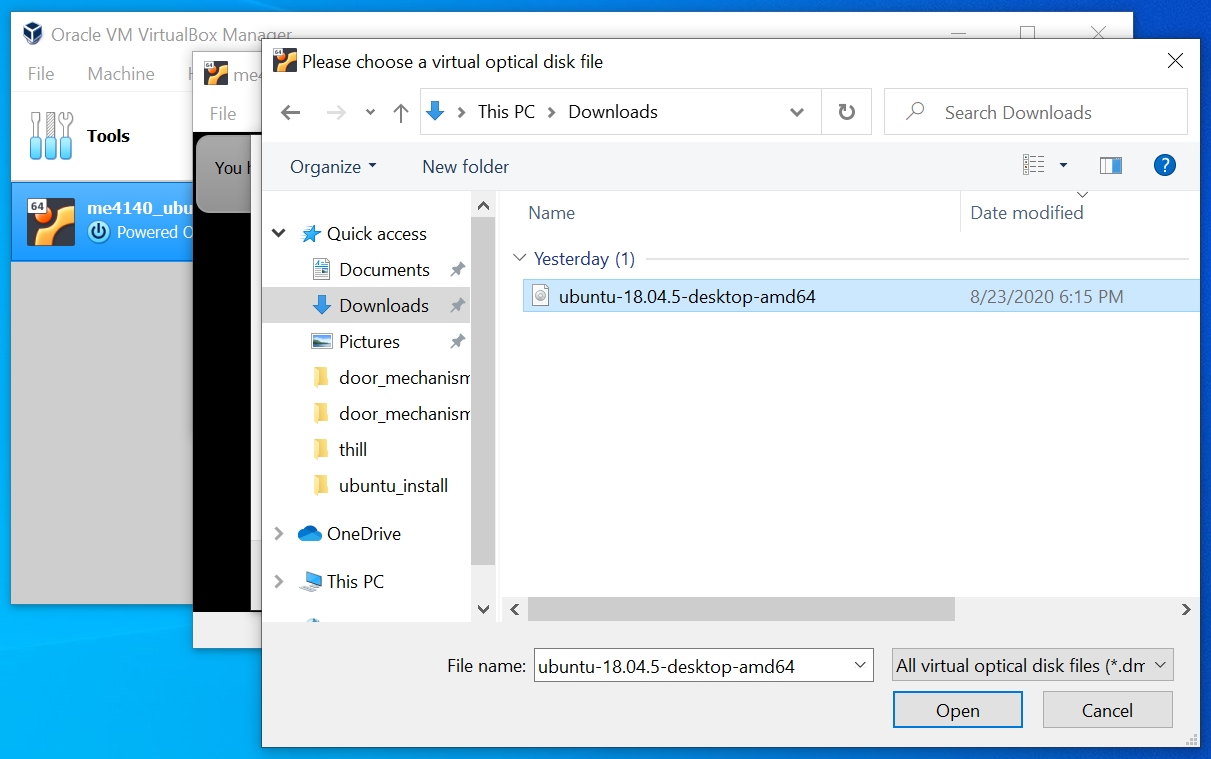
\includegraphics[scale=.6]{Capture11.png} \\
               \begin{itemize}
                    
     
                \item choose the Ubuntu .iso file that you downloaded.
                \item it is recommended that the media is on the local machine
                \item click {\bf open}
                
            \end{itemize}
\vspace{10mm}
\item Boot Ubuntu Installation Image: \vspace{5mm} \\
      		\hspace*{-2.5cm}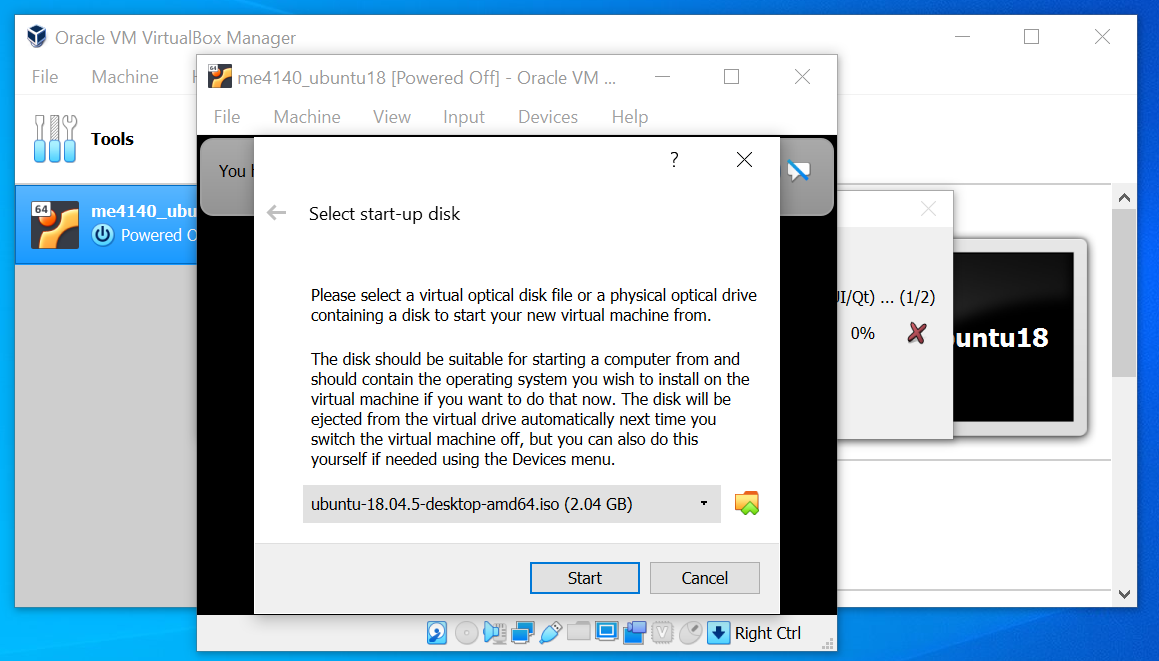
\includegraphics[scale=.6]{Capture12.png}
            \begin{itemize}
                    
                 \item click {\bf start}

            \end{itemize}

\newpage
\item Ubuntu Installation: \vspace{5mm} \\
      		\hspace*{-2.5cm}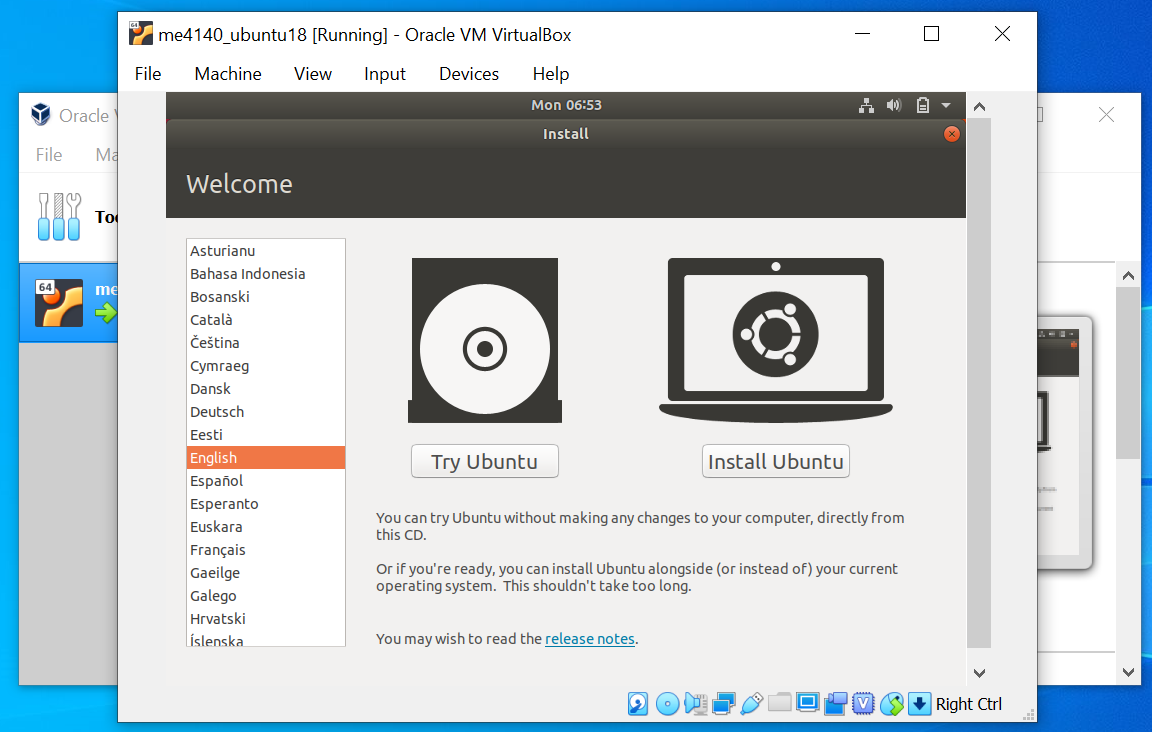
\includegraphics[scale=.6]{Capture13.png} 
            \begin{itemize}
               
                 \item click {\bf Install Ubuntu} (harmless if using VirtualBox)
                 \item try is for temporary or single session
                   
%                    \item check that you meet the requirements
%                 \item click the two check boxes for proprietary drivers
            \end{itemize}
\vspace{10mm}
\item Ubuntu Installation: \vspace{5mm} \\
      		\hspace*{-2.5cm}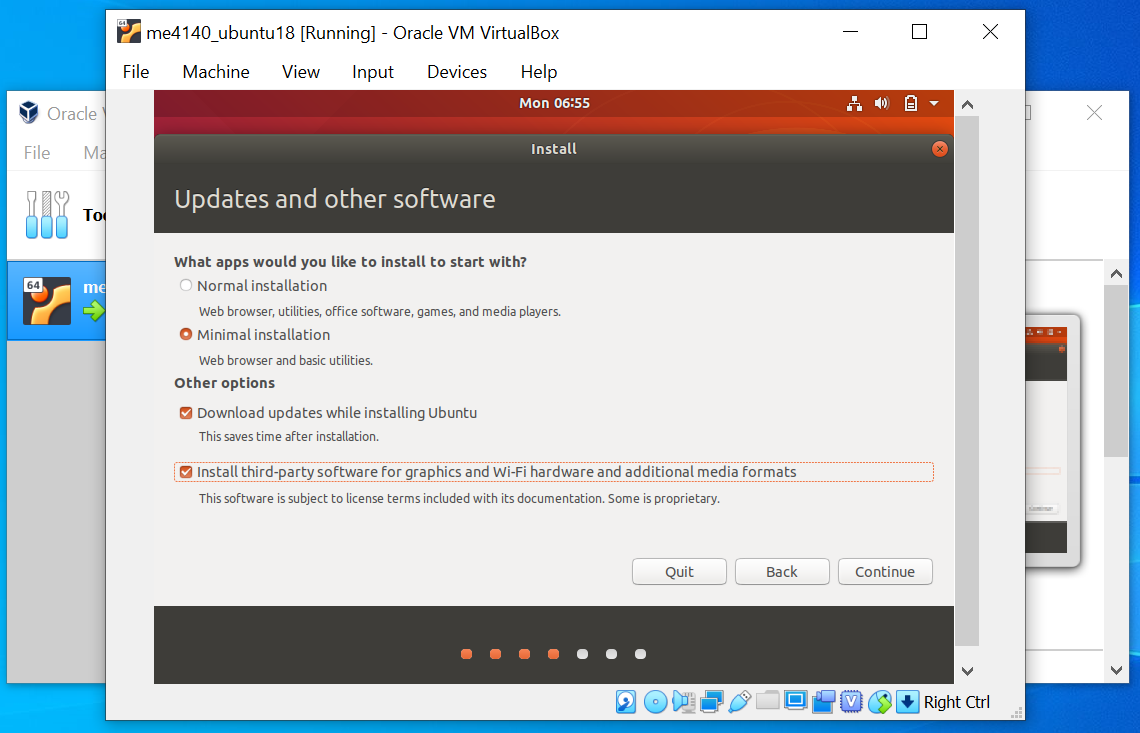
\includegraphics[scale=.6]{Capture15.png}\\
             \begin{itemize}
                    
                 \item choose {\bf Minimal Installation}
                 \item choose {\bf Download Updates...}           
                 \item choose {\bf Install third-party software...}  
                 \item click {\bf continue}     
            \end{itemize}

\vspace{5mm} 
\newpage
\item Ubuntu Installation: \vspace{5mm} \\
      		\hspace*{-2.5cm}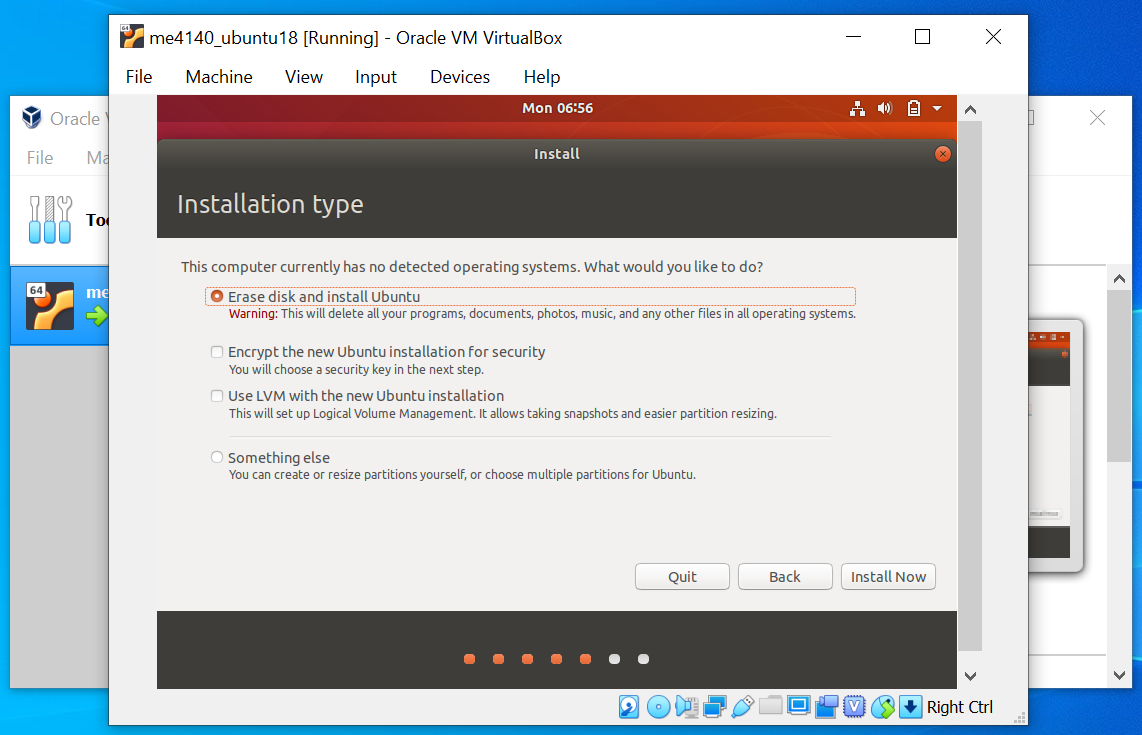
\includegraphics[scale=.6]{Capture16.png}\\
             \begin{itemize}
                    
                 \item choose {\bf Erase Everything and Install Ubuntu} 
                 \item this is {\B HARMLESS IF INSIDE VIRTUALBOX}
                 \item this is {\R DANGEROUS AND PERMANENT IF NOT IN VIRTUALBOX}
                 \item click {\bf Install Now}

            \end{itemize}

\vspace{5mm} 
\item Confirm Hard drive partitioning: \vspace{5mm} \\
      		\hspace*{-2.5cm}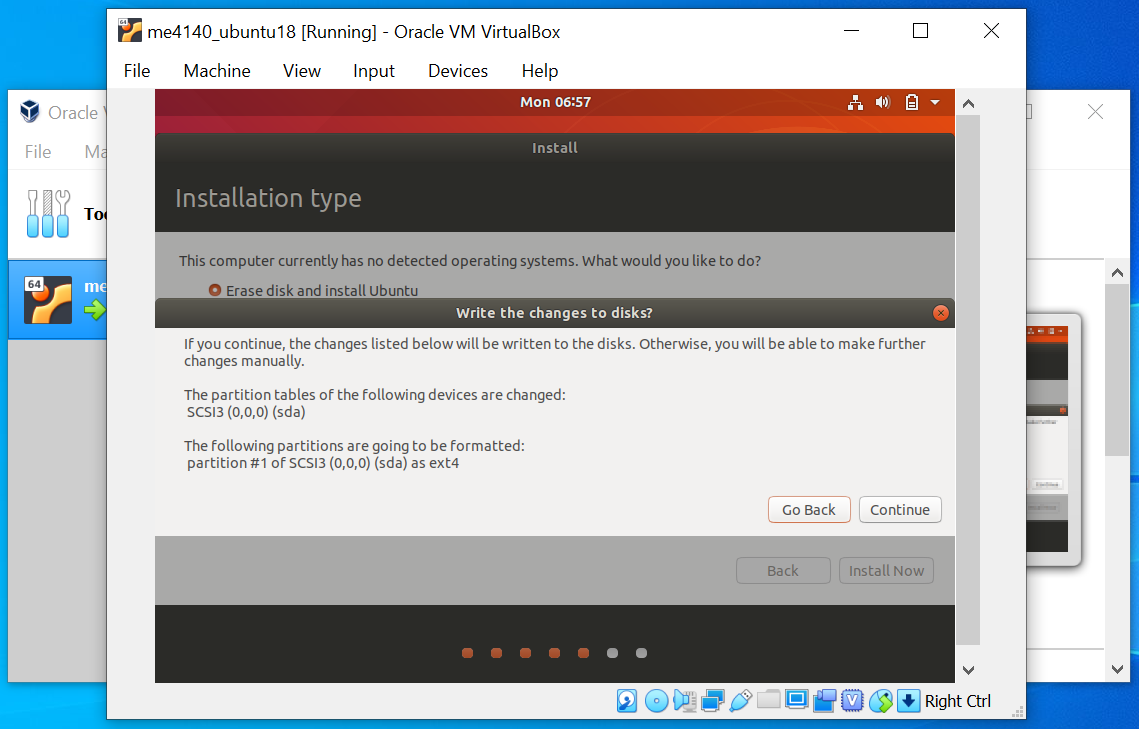
\includegraphics[scale=.6]{Capture17.png}
      		 \begin{itemize}
                    
                 \item you are confiming to partition your virtual hard drive 
                 \item this will not affect your files outside of VirtualBox
                 \item click {\bf continue}

            \end{itemize}
      		
	\newpage
\item Choose a timezone: \vspace{5mm} \\
      		\hspace*{-2.5cm}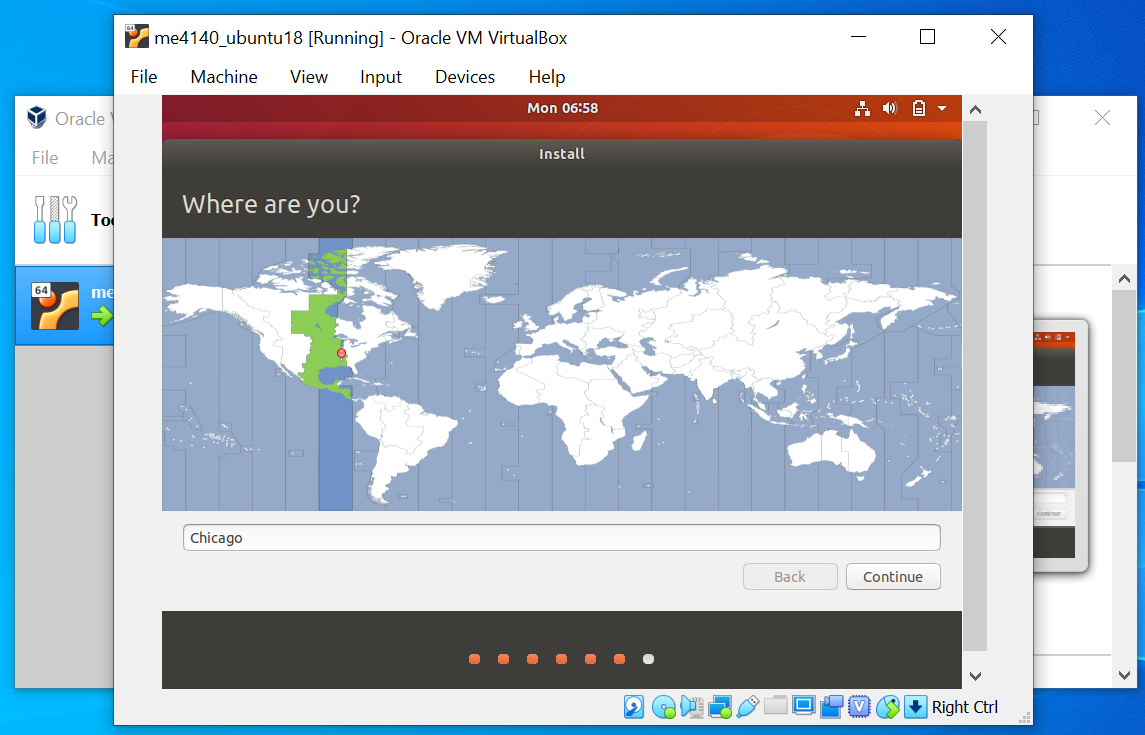
\includegraphics[scale=.6]{Capture18.png}\\
			

\vspace{5mm} 
\item Define you user settings: \vspace{5mm} \\
      		\hspace*{-2.5cm}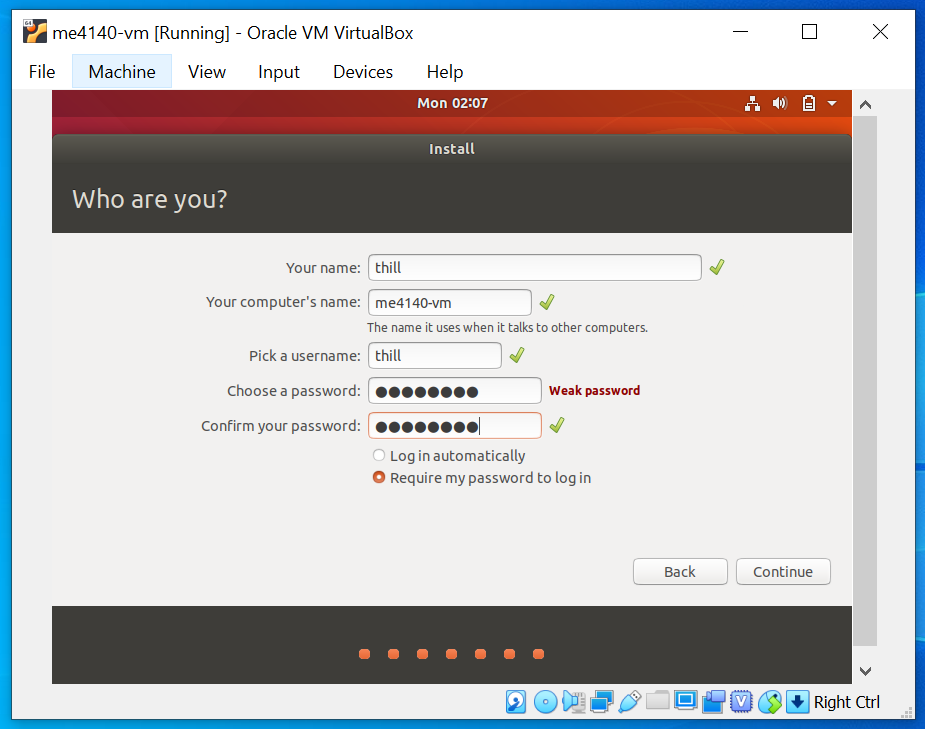
\includegraphics[scale=.6]{Capture19.png}
			\begin{itemize}
                 
				 \item choose a simple user name and computer name
				 \item choose a simple password or leave it blank
				 \item click {\bf continue}
                     
            \end{itemize}
\newpage
\item Wait for installation to complete: \vspace{5mm} \\
      		\hspace*{-2.5cm}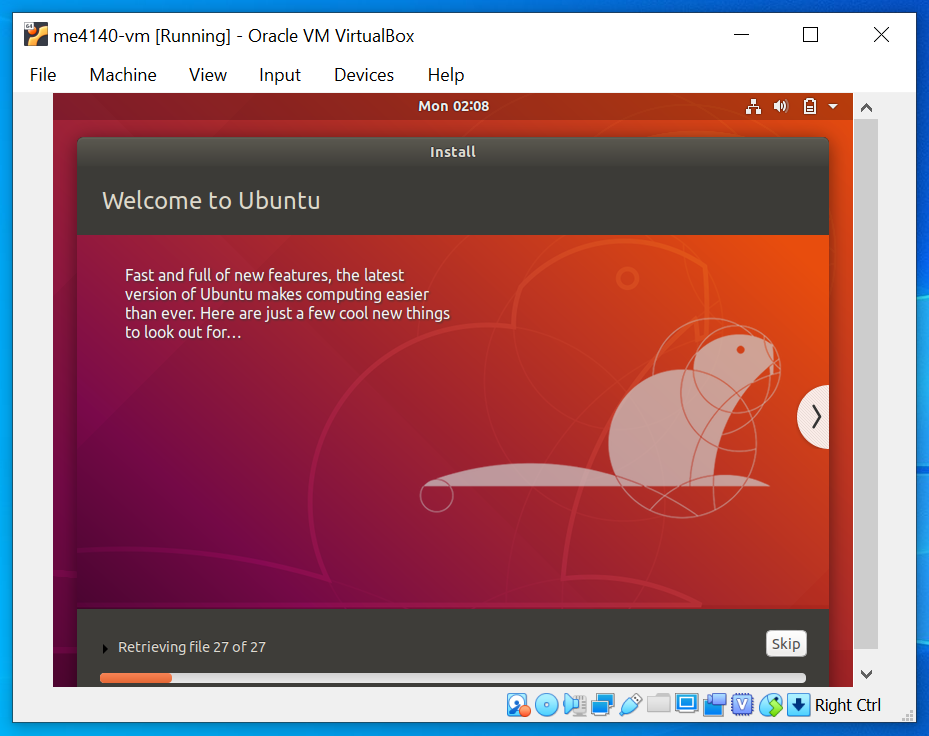
\includegraphics[scale=.6]{Capture20.png}
            \begin{itemize}
            \item  Make sure you are plugged into a power source or have a good battery
        \item  This will take several minutes depending on your system. Be patient, you are almost done! \vspace{5mm} \\
    \end{itemize} 

\vspace{5mm} 
\item Restart the VM: \vspace{5mm} \\
	\hspace*{-2.5cm}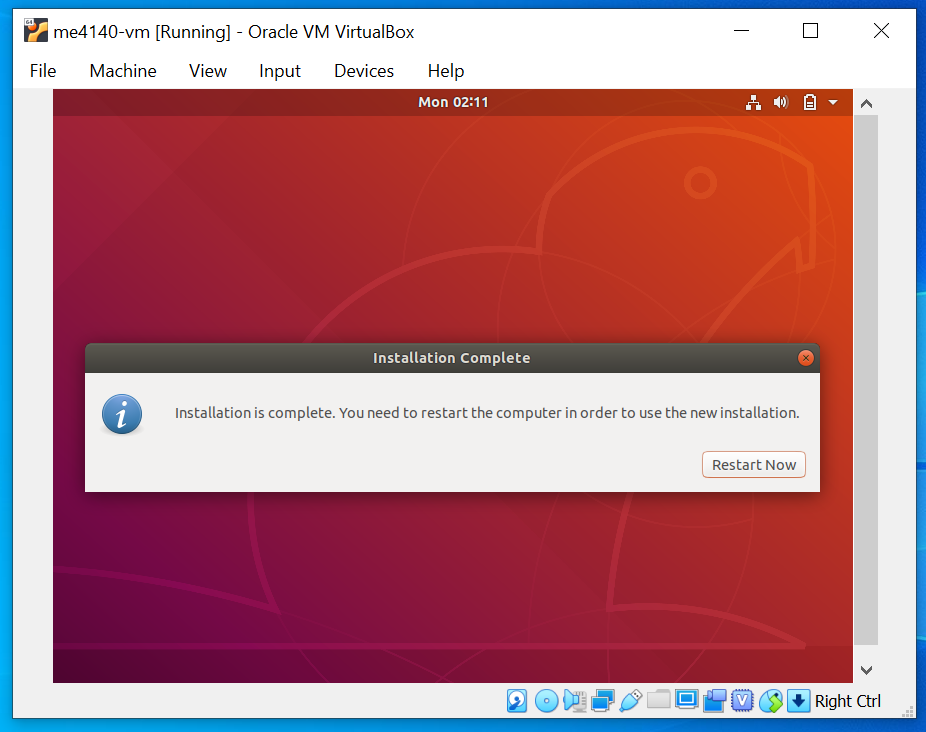
\includegraphics[scale=.6]{Capture21.png}  
    \begin{itemize}
        \item click {\bf Restart Now}
    \end{itemize}        

\newpage  

\item Restart to complete installation: \vspace{5mm} \\
      		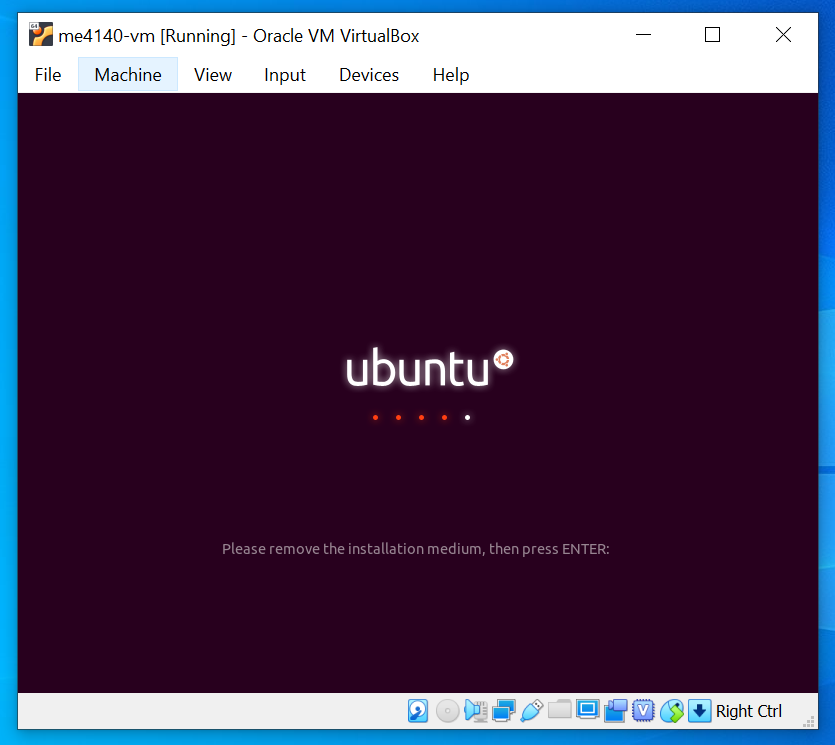
\includegraphics[scale=.55]{Capture22.png}
      		 \begin{itemize}
        	\item The installation of Ubuntu is now complete. Press the {\bf enter} key to shut down the machine. 
        	\item If it does not shut down click {\bf Machine $\rightarrow $ ACPI Shutdown}. 
    		\end{itemize}  
  \vspace{5mm}   		
    		\item Finally! Installation Complete: \vspace{5mm} \\
      		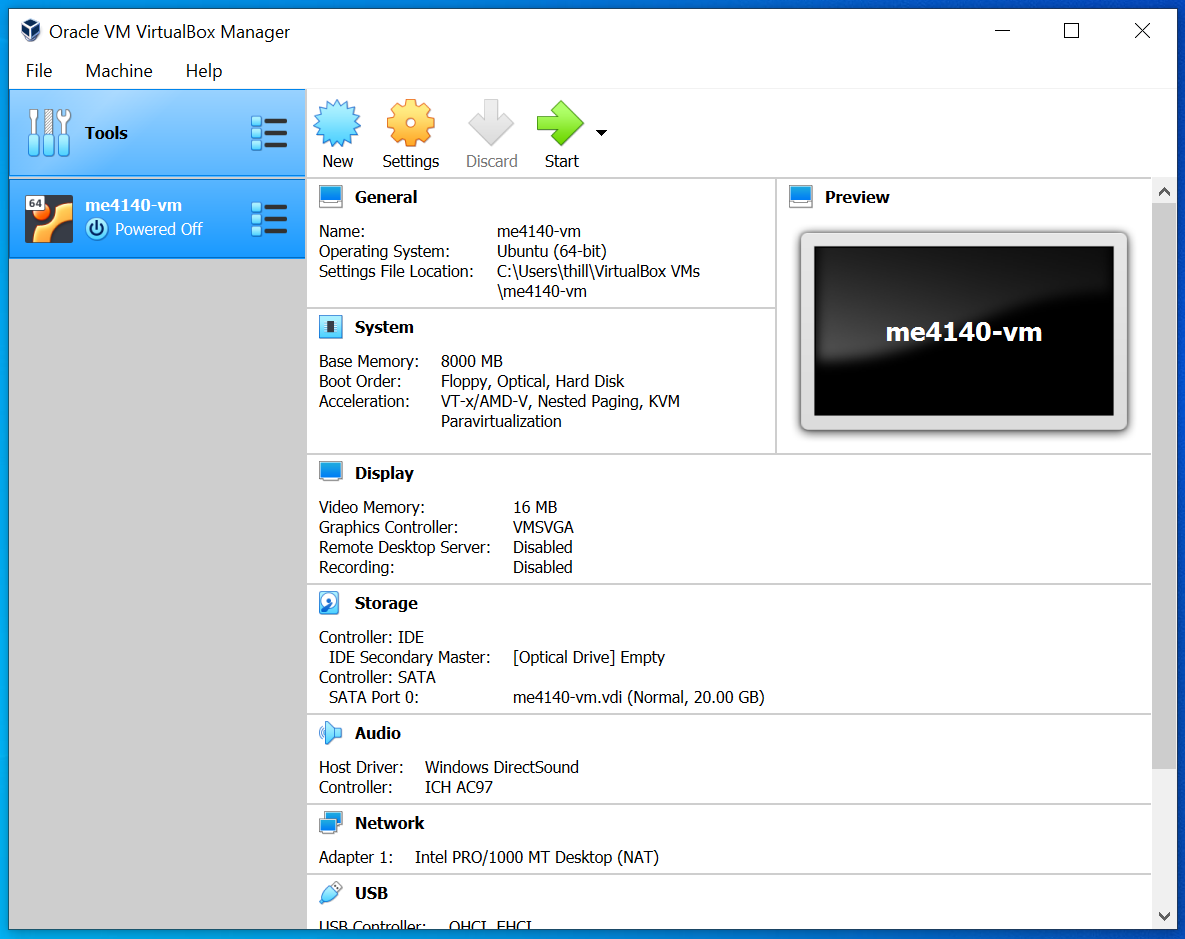
\includegraphics[scale=.55]{CaptureY.png}
      		 \begin{itemize}
        	\item You should now see your new virtual operating system in the list on the left. 
        	\item Click the {\bf start} button to turn it on. Login with the credential you created previously.
    		\end{itemize} 
    	
    	\newpage
    		\item Ubuntu Login Screen: \vspace{5mm} \\
      		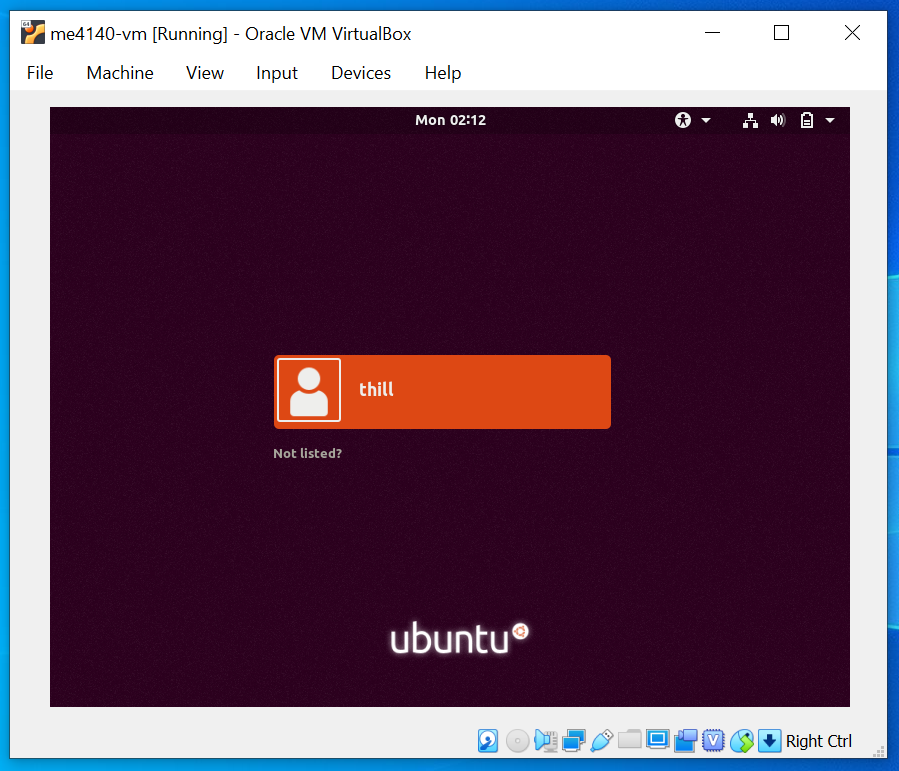
\includegraphics[scale=.55]{Capture23.png}
      		 \begin{itemize}
        	\item You should see the username you chose 
        	\item Login
    		\end{itemize} 
    		 \vspace{5mm} 
    		\item Ubuntu Welcome: \vspace{5mm} \\
      		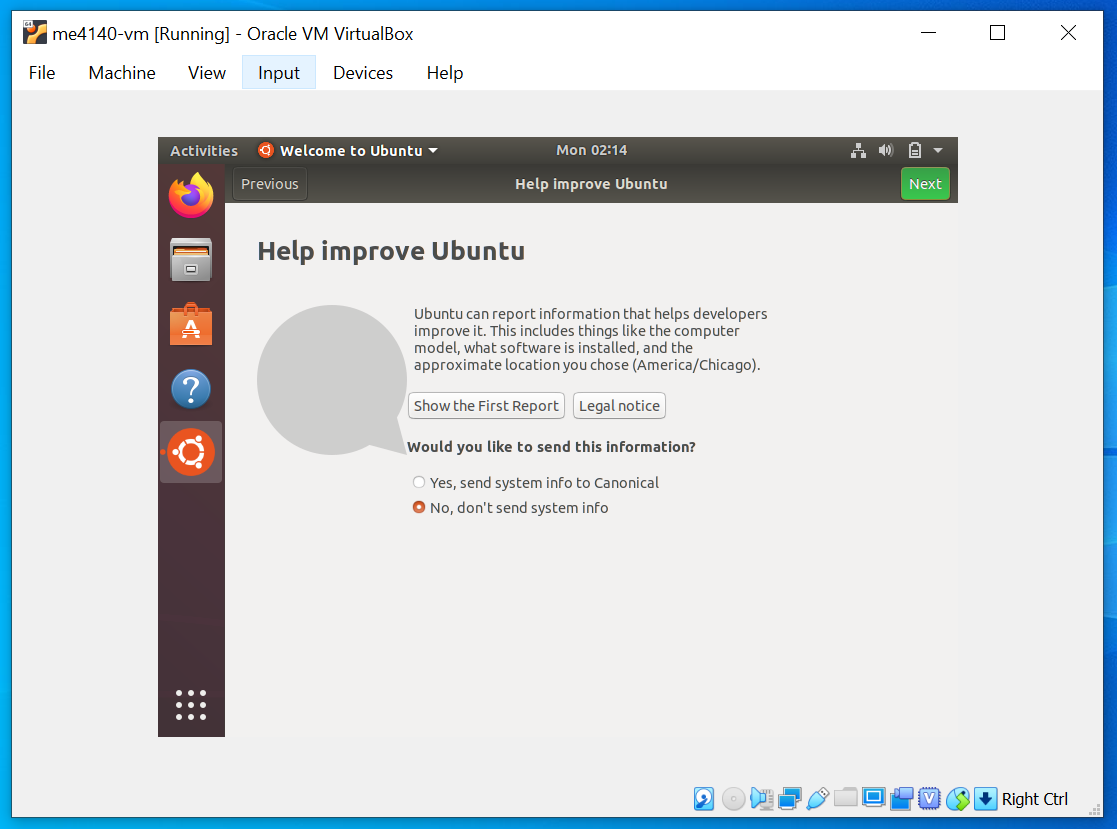
\includegraphics[scale=.55]{Capture24.png}
      		 \begin{itemize}      	
     		\item the default selections are fine
     		\item click {\bf next}
    		\end{itemize}
    		
    		\newpage
    		\item Fresh New Ubuntu - Bionic Beaver: \vspace{5mm} \\
      		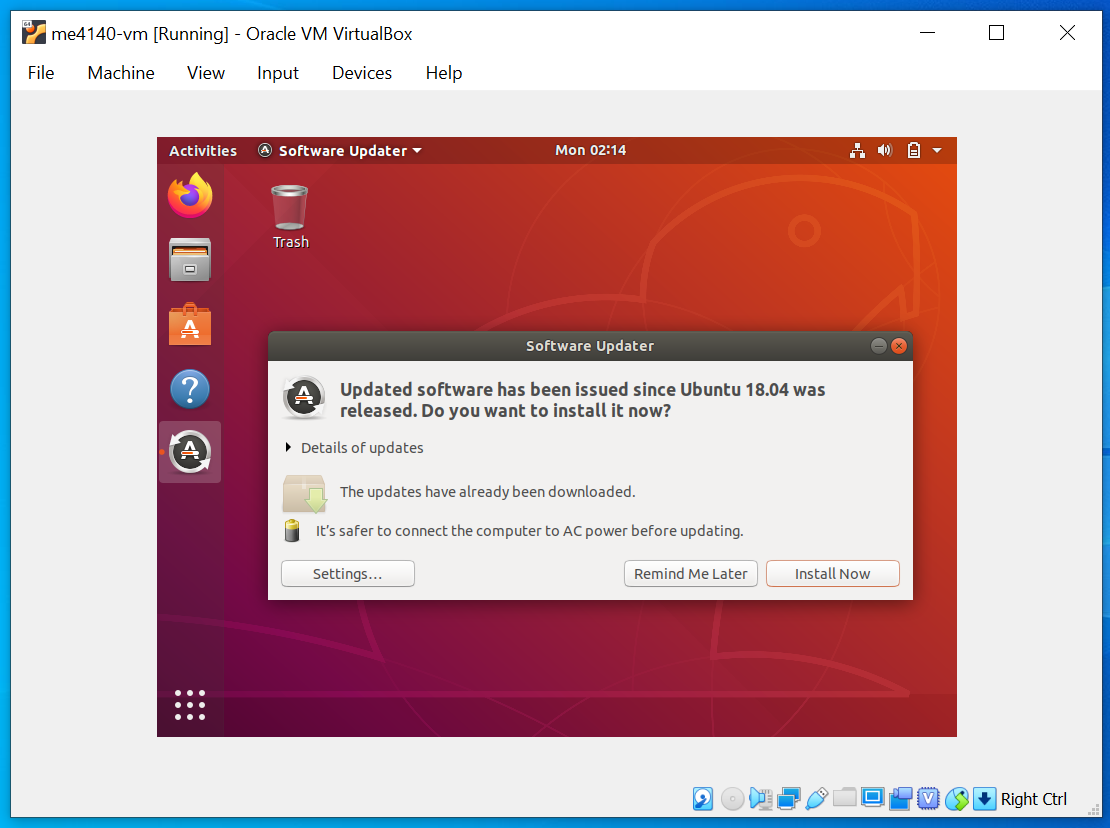
\includegraphics[scale=.55]{Capture25.png}
      		 \begin{itemize}
        	\item Install the updates. Do not upgrade to Ubuntu 20.
        	\item This requires the internet. You knew that. 
    		\end{itemize} 
    		 \vspace{5mm} 
    		\item Ubuntu Welcome: \vspace{5mm} \\
      		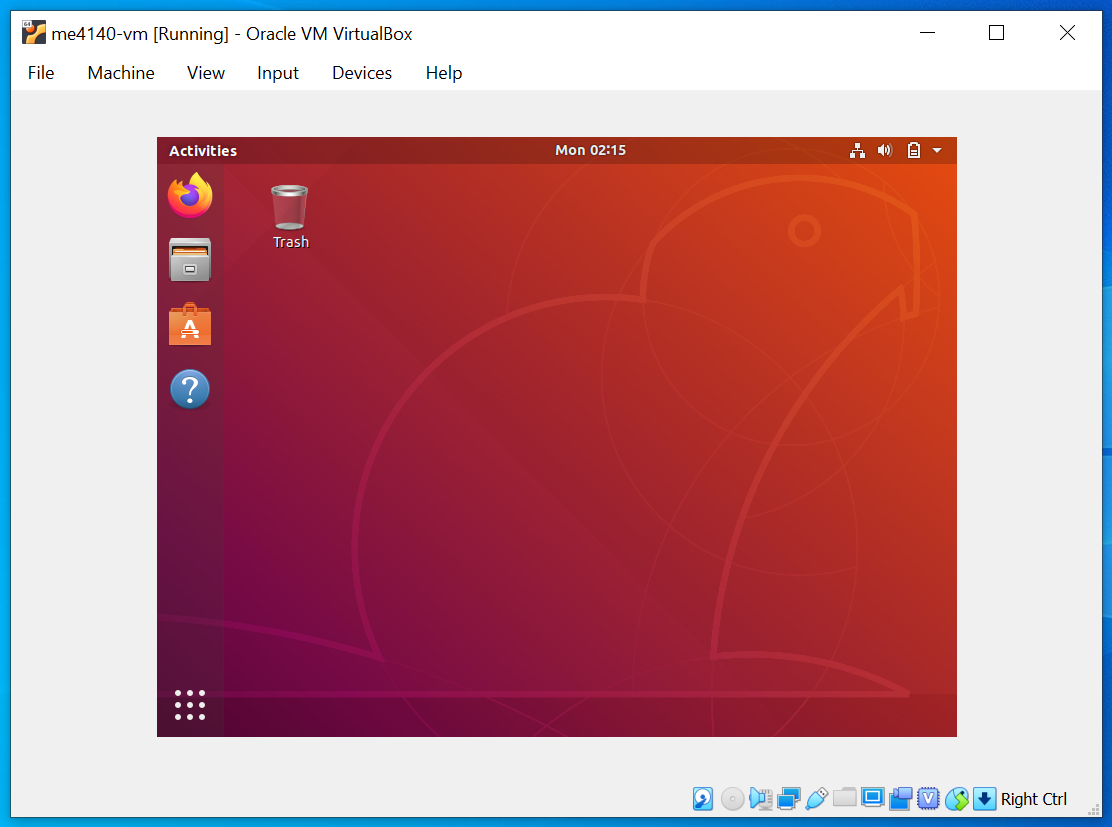
\includegraphics[scale=.55]{Capture26.png}
      		 \begin{itemize}
      		\item Now, it is a good idea to make a {\it backup} of your fresh install. VirtualBox can do this for you but you have to shut it down first.  
         
     		\item Find the {\bf shutdown} button in Ubuntu. You can also use the ACPI shutdown button in VirtualBox. Also, an unexpected shutdown should not hurt the system unless it is updating at the time, and if that happens it can usually repair itself. 
    		\end{itemize}
    		
    		\newpage
    		\item Fresh New Ubuntu - Bionic Beaver: \vspace{5mm} \\
      		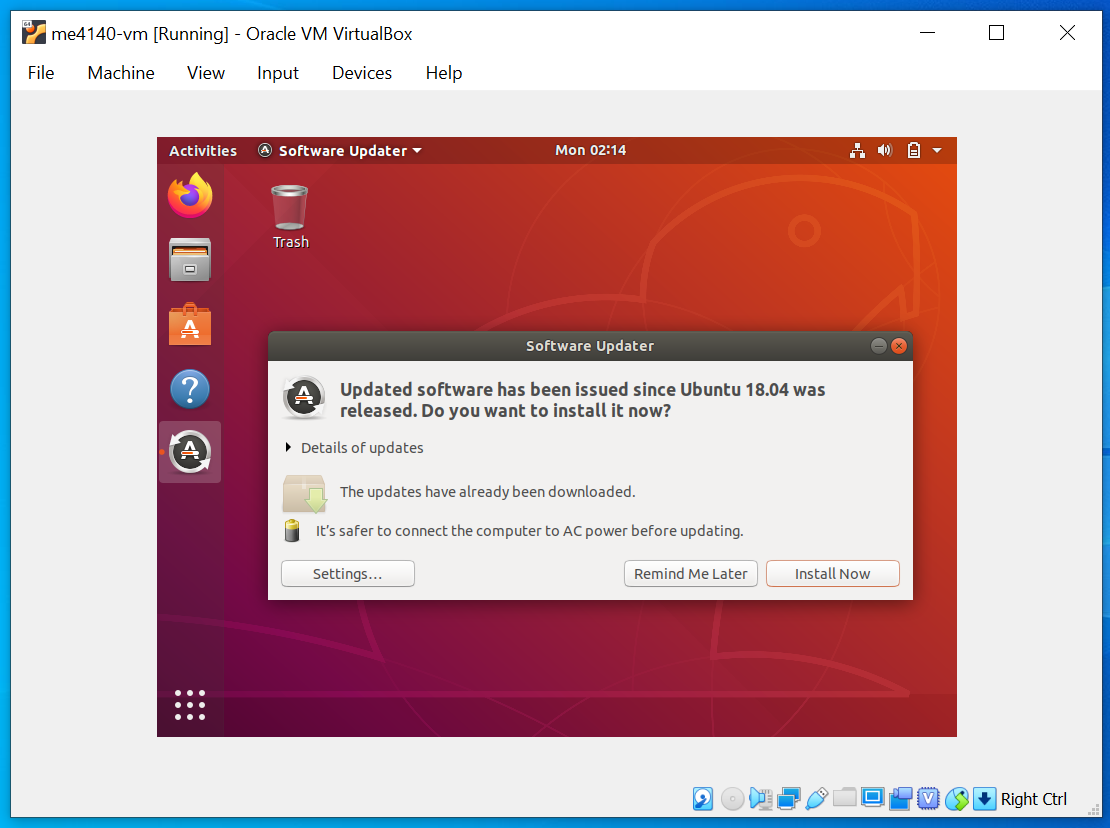
\includegraphics[scale=.55]{Capture25.png}
      		 \begin{itemize}
        	\item Install the updates. Do not upgrade to Ubuntu 20.
        	\item This requires the internet. You knew that. 
    		\end{itemize} 
    		 \vspace{5mm} 
    		\item Ubuntu Welcome: \vspace{5mm} \\
      		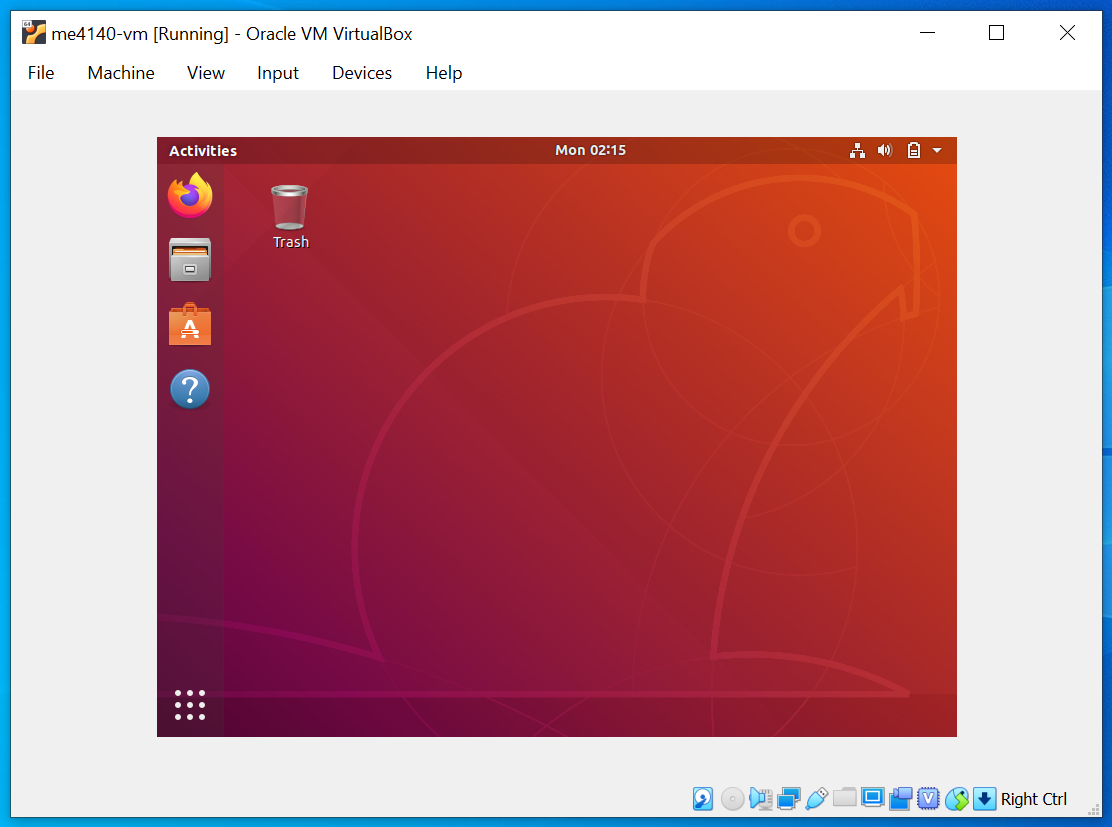
\includegraphics[scale=.55]{Capture26.png}
      		 \begin{itemize}
      		\item Now, it is a good idea to make a {\it backup} of your fresh install. VirtualBox can do this for you but you have to shut it down first.  
         
     		\item Find the {\bf shutdown} button in Ubuntu. You can also use the ACPI shutdown button in VirtualBox. Also, an unexpected shutdown should not hurt the system unless it is updating at the time, and if that happens it can usually repair itself. 
    		\end{itemize}
    		
    		\newpage
    		\item Back to VirtualBox : \vspace{5mm} \\
      		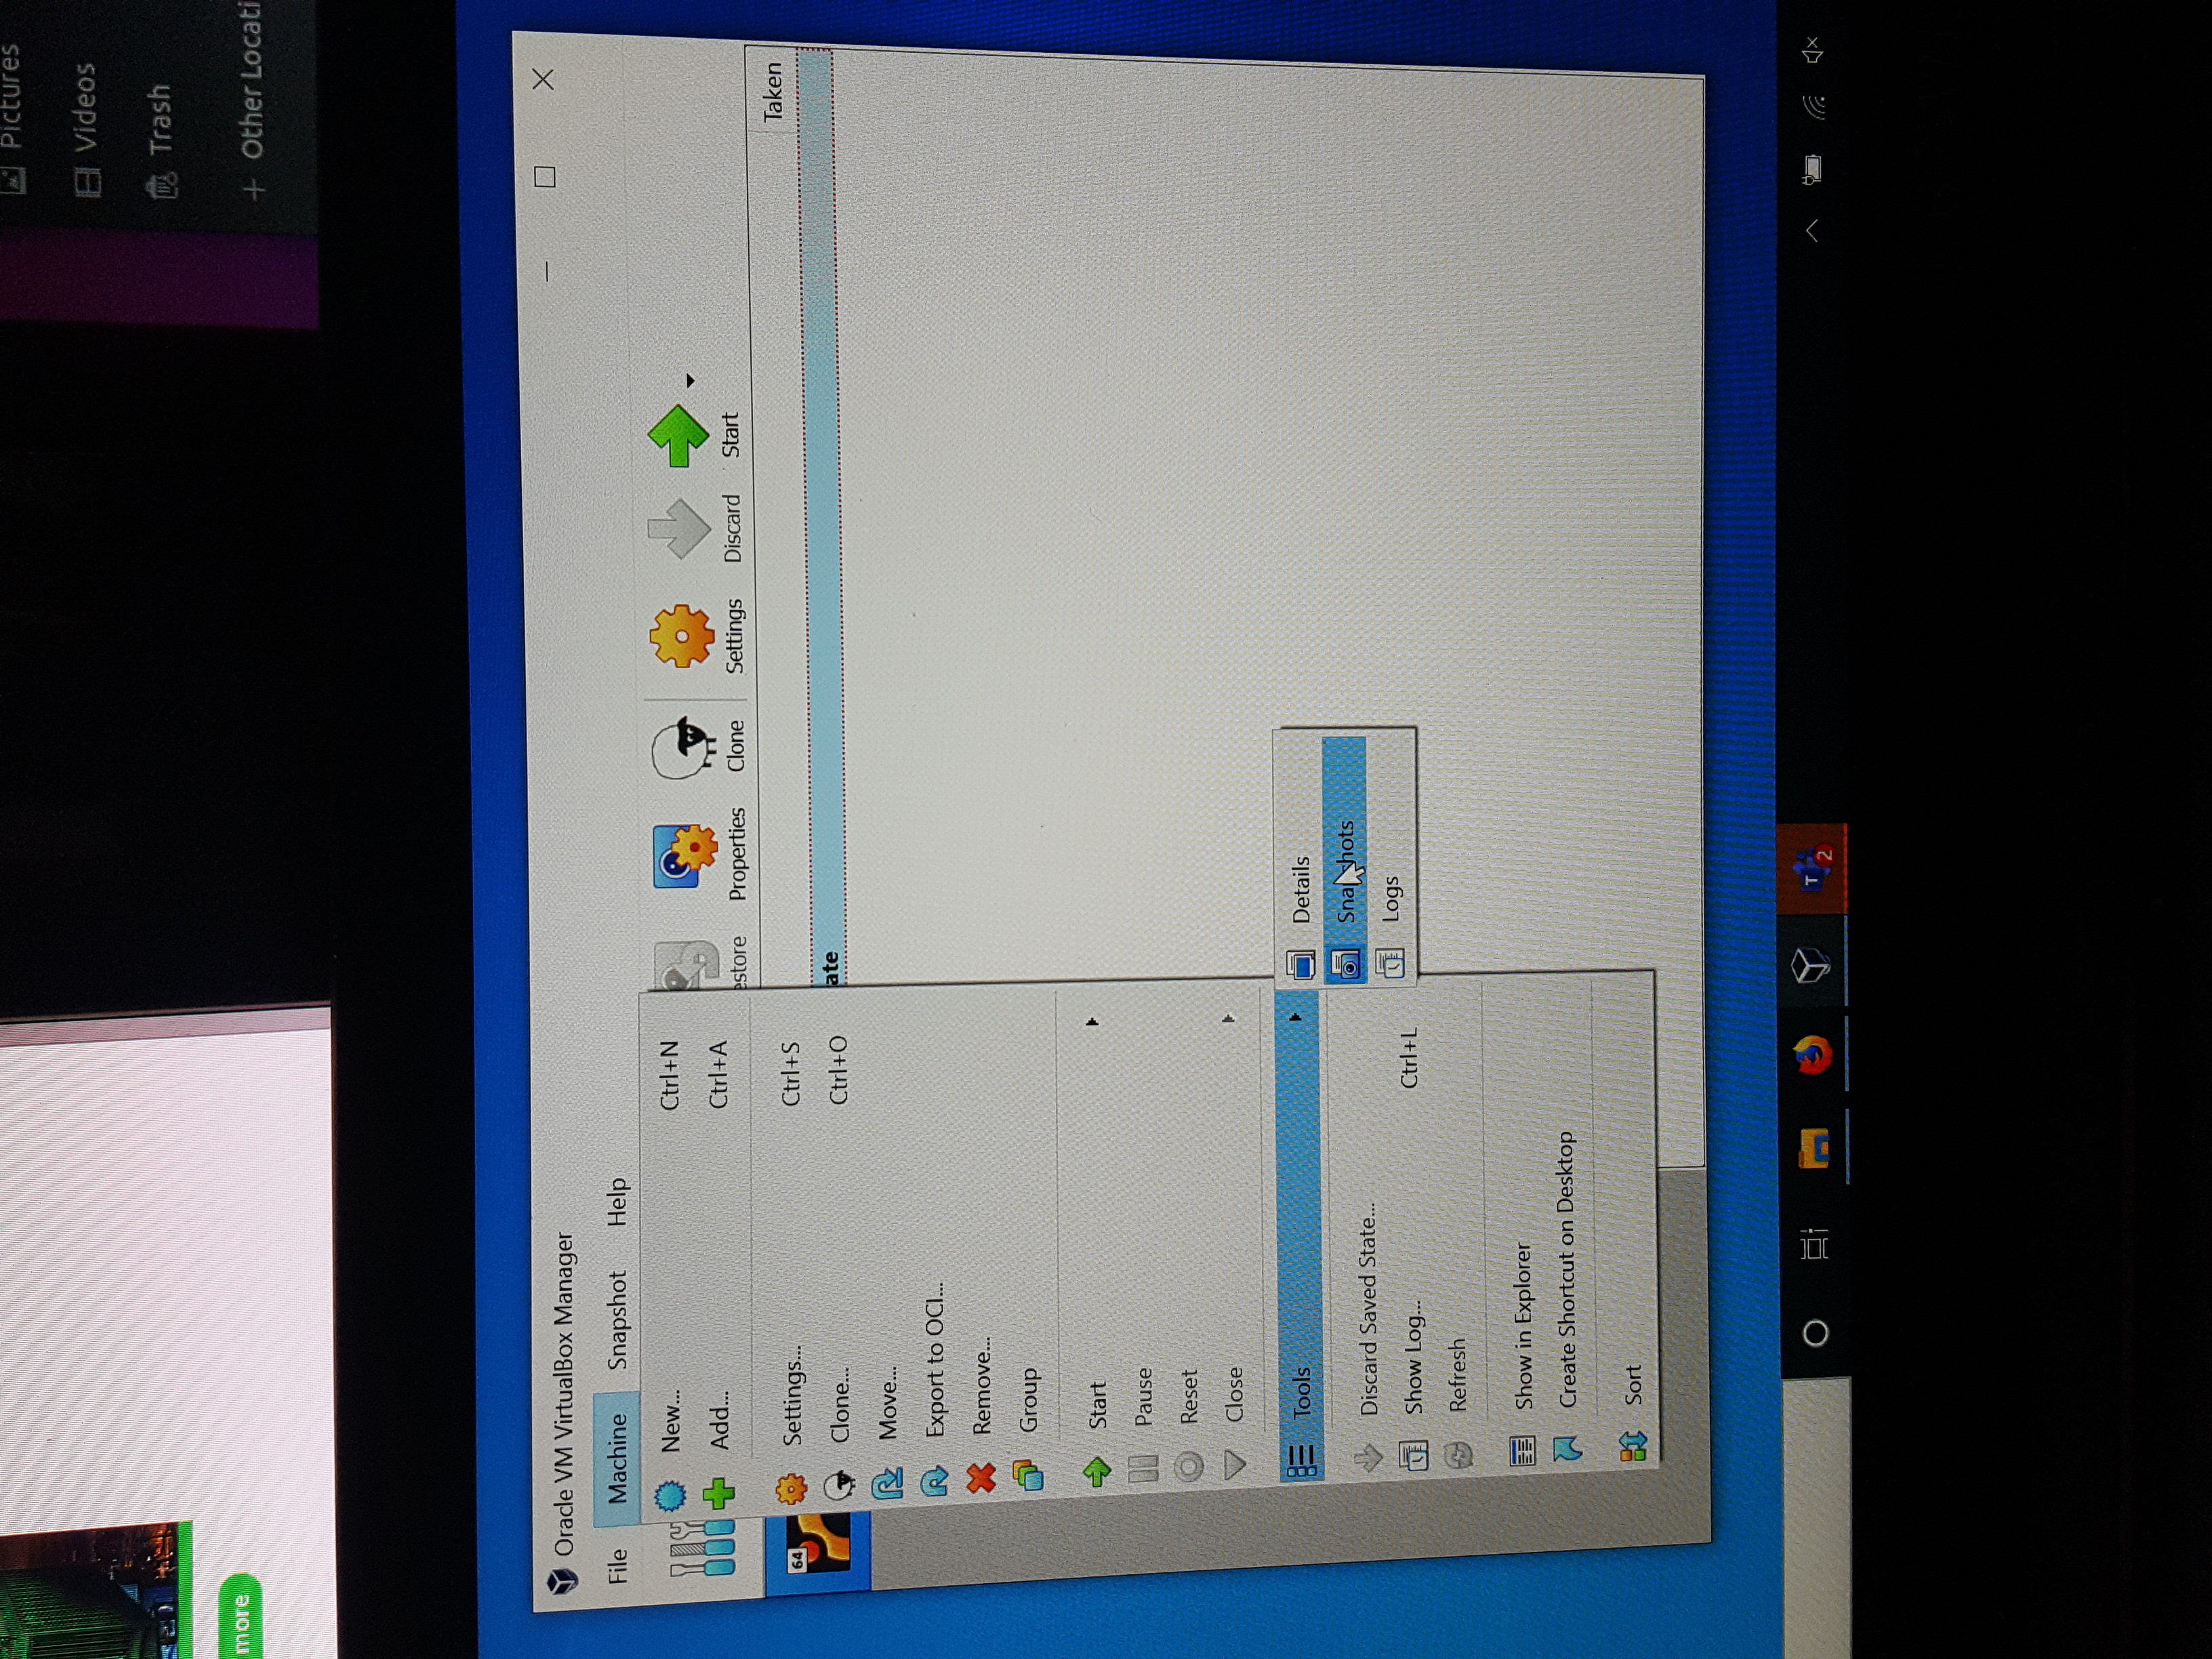
\includegraphics[scale=.120]{CaptureZ.png}
      		 \begin{itemize}
        	\item Select your new VM so that it is highlighted blue
        	\item click {\bf Machine \textgreater Tools \textgreater Snapshots} 
    		\end{itemize} 
    		 \vspace{5mm} 
    		 
    		\item Take a Snapshot for Backup: \vspace{5mm} \\
      		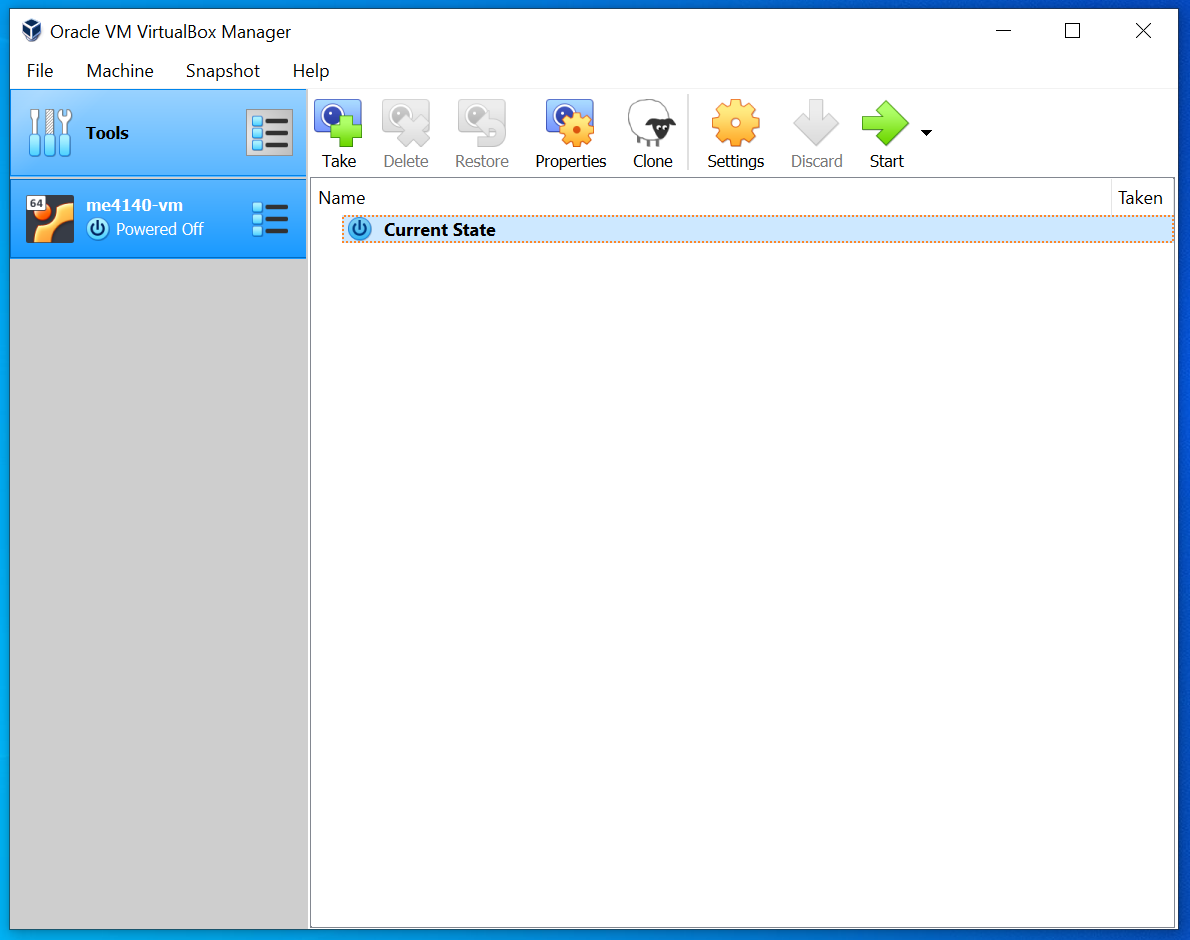
\includegraphics[scale=.50]{Capture27.png}
      		 \begin{itemize}
      		\item Snapshots can be used as a backup. This will save you all those steps if you if you ever need to start over.  
         
     		\item click {\bf Take} to save a snapshot of the current state of your virtual machine. Whew... that was a lot. 
     		\item Welcome to the world of Linux. Have fun!
    		\end{itemize}
\end{enumerate}

\end{description}    
\end{description}
\end{document}

